\section{Конструкториский раздел}
Для создания системы необходимо определиться с её структурой и теми возможностями, которые она будет обеспечивать при накладываемых на неё ограничениях. 
В первую очередь следует определить формат данных в рамках предметной области, а также задать описание функционирования программы. 
Кроме того, необходимо задать перечень алгоритмов и подходов к ним, что позволит определиться с выбором конкретных из них, наиболее подходящих для реализации заданной цели.

\subsection{IDEF0}
Для описания функционирования программы можно использовать графическую нотацию IDEF0. 
IDEF0-диаграмма разрабатываемой системы приведена на рисунках \ref{fig:2}, \ref{fig:3}.

% TODO: \usepackage{graphicx} required
\begin{figure}[H]
	\centering
	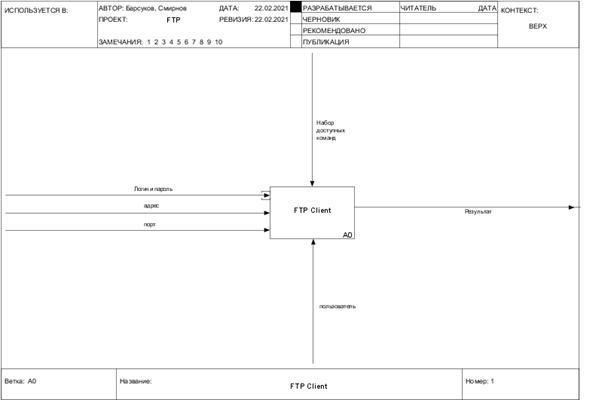
\includegraphics[width=0.7\linewidth]{src/img/2}
	\caption{A0}
	\label{fig:2}
\end{figure}

Общая концепция состоит в следующая: пользователь указывает необходимые данные для подключения и устанавливается соединение с ftp сервером через связанный сокет. 
После этого программа ожидает ввод команды и отправляет запрос  на сервер после этого ждет ответ и выводит результат на экран до тех пока пользователь не завершит работу.

% TODO: \usepackage{graphicx} required
\begin{figure}[H]
	\centering
	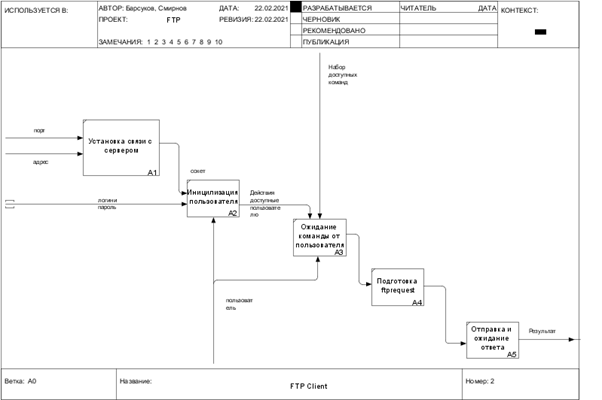
\includegraphics[width=0.7\linewidth]{src/img/3}
	\caption{A0 детально}
	\label{fig:3}
\end{figure}




\subsection{Описание структуры разрабатываемой программы}
Для разрабатываемой программы необходимо выделить хранимые данные, общий подход к структуре программного продукта, а также конкретизировать формат работы 
модулей.

На рисунках \ref{fig:4}, \ref{fig:5} представлены прототипы используемых в работе классов. 
Рисунок \ref{fig:4} показывает прототип класса Socket, представляющий из себя обертку вокруг <sys/socket>. 
Предоставляет следующие атрибуты и методы:
\begin{enumerate}
	\item Методы: \begin{enumerate}
		\item Socket() - конструктор без аргументов. Иницилизирует \_addr = 0 \_sockfd = -1;
		\item is\_valid() - проверяет файловый дескриптор;
		\item fd() - возвращает файловый дескриптор;
		\item fd(int \_fd) - устанавливает значение fd;
		\item port() - возвращает порт ;
		\item host() - возвращает адрес хоста;
		\item create() - создает файловый дескриптор сокета;
		\item bind(int port) - привязывает сокет к порту;
		\item connect(int ip, int port) - связывает сокет с удаленным сервером;
		\item listen() - ставит сокет на ожидание;
		\item aссept() - Функция accept ожидает запрос на установку TCP-соединения от удаленного хоста. В качестве аргумента ей передается дескриптор слушающего сокета;
		\item recv() - получает ответ от связанного сокета;
		\item close() - освобождает ресурсы дескриптора сокета
	\end{enumerate}
	\item Атрибуты:
		\begin{enumerate}
			\item \_sockfd - дескриптор сокета;
			\item \_addr - представляет из себя структуру хранящую в себе адрес, порт и семейсво
		\end{enumerate}
\end{enumerate}

Также на рисунке \ref{fig:4} представлен сокет clientSocket класс который будет представлять из себя конкретную реализацию сокета используемого в нашем клиенте.

% TODO: \usepackage{graphicx} required
\begin{figure}[H]
	\centering
	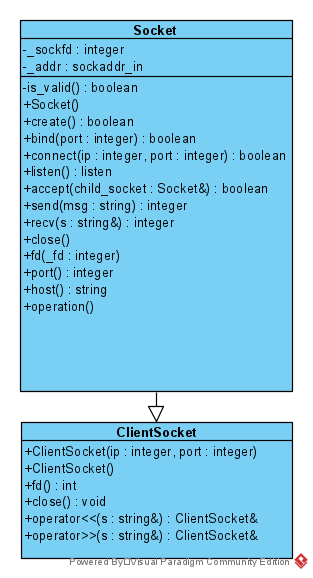
\includegraphics[width=0.7\linewidth]{src/img/4}
	\caption{Диаграмма Socket и СlientSocket}
	\label{fig:4}
\end{figure}

% TODO: \usepackage{graphicx} required
\begin{figure}[H]
	\centering
	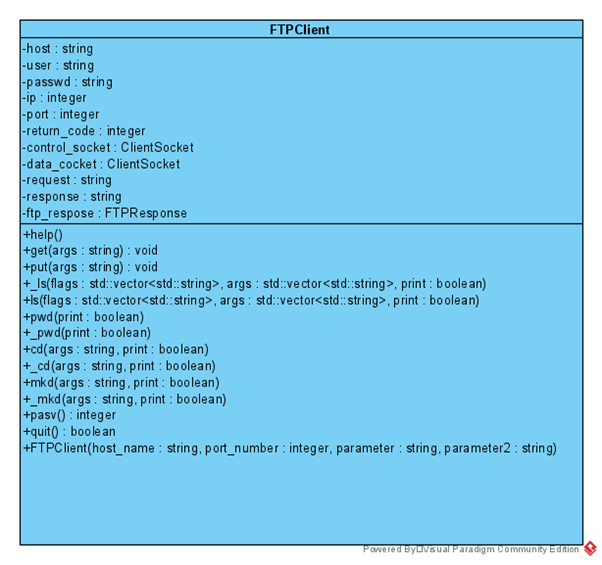
\includegraphics[width=0.7\linewidth]{src/img/5}
	\caption{Диаграмма FTPClient}
	\label{fig:5}
\end{figure}

На рисунке \ref{fig:5} изображен прототип FTPClient класса, который реализует основную логику взаимодействия пользователя с клиентом.

